\documentclass[12pt,a4paper]{article}

% --- Csomagok betöltése ---
\usepackage[utf8]{inputenc}
\usepackage[T1]{fontenc}
\usepackage[magyar]{babel}
\usepackage{amsmath, amssymb}
\usepackage{tikz}
\usepackage{geometry}
\usepackage{xcolor}

% --- Margók beállítása ---
\geometry{top=2.5cm, bottom=2.5cm, left=2.5cm, right=2.5cm}

% --- SZÍNEK ÉS EGYÉB BEÁLLÍTÁSOK ---
\definecolor{bvred}{rgb}{0.8, 0.0, 0.0}
\newcommand{\textbfr}[1]{\textbf{\textcolor{bvred}{#1}}}

% --- Dokumentum kezdete ---

%%% Megjelenítéshez automatikusan kiegészített csomagok %%%
\usepackage{amsfonts, amsthm}
\usepackage{tcolorbox}
\tcbuselibrary{theorems,skins,breakable}
\usepackage{pgfplots}
\pgfplotsset{compat=1.18}
\usepackage{graphicx}
\usepackage{enumitem}
\usepackage{booktabs}
\usepackage{float}
\usepackage{caption}
\usepackage{microtype}

\usepackage{hyperref}
\author{}

\begin{document}

% --- CÍM ---
\title{\textbfr{Deriválási szabályok}\\[0.5ex]
\large Alapozás: Deriválás, monotonitás, szélsőérték és konvexitás kapcsolata}
\author{Készítette:\\Varga Dávid}
\date{}
\maketitle

Mielőtt egy teljes függvényvizsgálatot elvégeznénk, elengedhetetlen, hogy biztos alapokon nyugodjon a differenciálszámítás és a függvények geometriai tulajdonságai közötti kapcsolat. A deriváltak nem csupán elvont algebrai formulák, hanem hatékony eszközök, amelyekkel a függvény ,,viselkedését'' – növekedését, csökkenését, görbületét és szélsőértékeit – térképezhetjük fel. 

Ebben a fejezetben megvizsgáljuk, hogyan árulja el az első és a második derivált egy függvény grafikonjának legfontosabb titkait.

\section*{1. Az első derivált és a monotonitás}

Tudjuk, hogy egy $f(x)$ függvény differenciálhányadosa egy adott $x_0$ pontban geometriailag a függvény grafikonjához húzott érintő meredekségét adja meg. Ha ez a meredekség pozitív, a függvény grafikonja emelkedik; ha negatív, a grafikon süllyed. Ezt az intuitív elképzelést precíz matematikai formába is önthetjük.

\textbf{Definíció.} \textit{Tegyük fel, hogy az $f(x)$ függvény differenciálható egy $(a,b)$ nyílt intervallumon. Ha minden $x \in (a,b)$ esetén $f'(x) > 0$, akkor a függvény az intervallumon \textcolor{bvred}{szigorúan monoton növekvő}. Ha minden $x \in (a,b)$ esetén $f'(x) < 0$, akkor az intervallumon a függvény \textcolor{bvred}{szigorúan monoton csökkenő}.}

Az összefüggés logikája világos: az első derivált előjele közvetlenül meghatározza a függvény haladási irányát. Ha a vizsgált tartományban az érintők irányszöge hegyesszög (pozitív tangens), a függvényértékek egyre nagyobbak lesznek.

\section*{2. Lokális szélsőértékek keresése}

A monotonitás változása szorosan kötődik a hegycsúcsokhoz (maximumok) és völgyekhez (minimumok). Képzeljünk el egy hegymászót, aki felér a csúcsra: felfelé haladt (növekvő szakasz), majd mielőtt elindulna lefelé (csökkenő szakasz), egyetlen pillanatra vízszintes terepen áll. Ekkor az érintő meredeksége nulla.

\textbf{Definíció.} \textit{Az $f(x)$ függvénynek egy $x_0$ pontban \textcolor{bvred}{lokális szélsőértéke} (maximuma vagy minimuma) van, ha létezik a pontnak olyan környezete, ahol a függvényértékek egyike sem nagyobb (maximum esetén) vagy nem kisebb (minimum esetén), mint az $f(x_0)$ érték.}

\textbf{Definíció.} \textit{Azt az $x_0$ pontot, ahol az első derivált értéke nulla, azaz $f'(x_0) = 0$, a függvény \textcolor{bvred}{stacionárius pontjának} nevezzük.}

Fontos azonban tisztázni, hogy a stacionárius pont létezése \textit{szükséges}, de \textit{nem elégséges} feltétele a szélsőértéknek. Egy pontban pontosan akkor van szélsőérték, ha az első derivált nulla (vagy nem létezik), \textbf{és} az első derivált a pontban \textbf{előjelet vált}.

Vizsgáljuk meg a lehetséges eseteket stacionárius pont ($f'(x_0) = 0$) környezetében:
\begin{itemize}
    \item \textbf{Lokális maximum:} Ha $x < x_0$ esetén $f'(x) > 0$ (nő), és $x > x_0$ esetén $f'(x) < 0$ (csökken), a függvénynek lokális maximuma van.
    \item \textbf{Lokális minimum:} Ha $x < x_0$ esetén $f'(x) < 0$ (csökken), és $x > x_0$ esetén $f'(x) > 0$ (nő), a függvénynek lokális minimuma van.
    \item \textbf{Nincs szélsőérték:} Ha az első derivált \textit{nem vált előjelet} (például végig pozitív, mint az $f(x)=x^3$ esetében az origóban), akkor a pont egy "vízszintes inflexiós pont", de nem szélsőérték.
\end{itemize}

\section*{3. A második derivált és a konvexitás}

Ahogy az első derivált a függvényérték ($y$) változási gyorsaságát méri, úgy a második derivált ($f''(x)$) az \textit{érintő meredekségének} ($f'(x)$) a változási gyorsaságát mutatja meg. Ha a meredekség egyre nő (például egy nagy negatív számból elindul a nulla felé, majd pozitív lesz), a függvény grafikonja "felfelé kunkorodik", tehát mosolyog.
\textbf{Definíció.} \textit{Tegyük fel, hogy az $f(x)$ függvény kétszer differenciálható egy $(a,b)$ intervallumon. Ha minden $x \in (a,b)$ esetén $f''(x) > 0$, akkor a függvény grafikonja \textcolor{bvred}{konvex} (alulról domború). Ha minden $x \in (a,b)$ esetén $f''(x) < 0$, akkor a grafikon \textcolor{bvred}{konkáv} (alulról homorú).}

A konvexitás nemcsak a görbület alakját árulja el, hanem a szélsőértékek besorolásában is gyors eszközt ad a kezünkbe (ez az úgynevezett \textit{második derivált teszt}):
\begin{align*}
    f'(x_0) = 0 \text{ és } f''(x_0) > 0 \quad &\Rightarrow \quad \text{Lokális \textbf{minimum} (a völgy alján vagyunk, görbület felfelé nyitott)} \\
    f'(x_0) = 0 \text{ és } f''(x_0) < 0 \quad &\Rightarrow \quad \text{Lokális \textbf{maximum} (a hegy csúcsán vagyunk, görbület lefelé nyitott)}
\end{align*}

\section*{4. Vizuális összefoglaló egy példán keresztül}

Tekintsük az $f(x) = x^3 - 3x$ függvényt. Ennek deriváltjai a következőképpen alakulnak:
\[
    f'(x) = 3x^2 - 3 = 3(x-1)(x+1)
\]
\[
    f''(x) = 6x
\]
A stacionárius pontok $f'(x)=0$ alapján $x_1 = -1$ és $x_2 = 1$. A második derivált teszt szerint $f''(-1) = -6 < 0$ (maximum), és $f''(1) = 6 > 0$ (minimum). Az inflexiós pont $f''(x)=0$ alapján $x = 0$.

\vspace{0.5cm}

\begin{center}
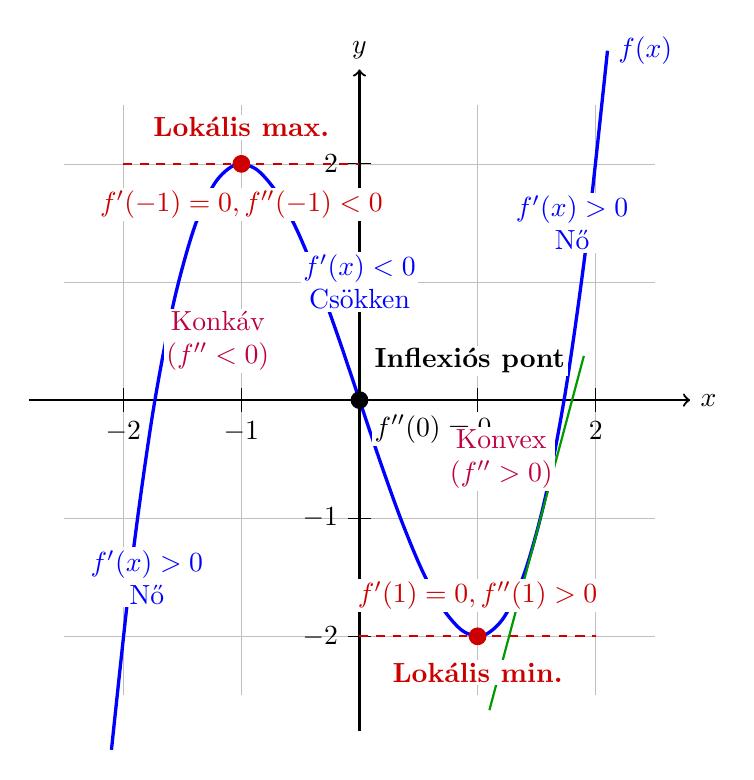
\begin{tikzpicture}[scale=1.5]
    % Rács és tengelyek
    \draw[lightgray, very thin, step=1] (-2.5, -2.5) grid (2.5, 2.5);
    \draw[->, thick] (-2.8, 0) -- (2.8, 0) node[right] {$x$};
    \draw[->, thick] (0, -2.8) -- (0, 2.8) node[above] {$y$};
    
    % Tengely feliratok
    \foreach \x in {-2, -1, 1, 2}
        \draw (\x, 0.1) -- (\x, -0.1) node[below] {$\x$};
    \foreach \y in {-2, -1, 1, 2}
        \draw (0.1, \y) -- (-0.1, \y) node[left] {$\y$};
        
    % A függvény rajzolása
    \draw[domain=-2.1:2.1, smooth, variable=\x, blue, very thick] plot ({\x}, {\x*\x*\x - 3*\x}) node[right] {$f(x)$};
    
    % Érintők rajzolása (stacionárius pontokban)
    % x = -1 helyen, y = 2
    \draw[domain=-2:0, smooth, variable=\x, bvred, dashed, thick] plot ({\x}, {2});
    % x = 1 helyen, y = -2
    \draw[domain=0:2, smooth, variable=\x, bvred, dashed, thick] plot ({\x}, {-2});
    
    % Egy érintő egy emelkedő szakaszon (x = 1.5)
    % f'(1.5) = 3*(1.5)^2 - 3 = 6.75 - 3 = 3.75
    % f(1.5) = (1.5)^3 - 3*1.5 = 3.375 - 4.5 = -1.125
    % y = 3.75*(x - 1.5) - 1.125 = 3.75*x - 5.625 - 1.125 = 3.75x - 6.75
    \draw[domain=1.1:1.9, smooth, variable=\x, green!60!black, thick] plot ({\x}, {3.75*\x - 6.75});
    
    % Pontok kiemelése
    \filldraw[bvred] (-1, 2) circle (2pt);
    \node[anchor=south, text=bvred, fill=white, inner sep=1pt] at (-1, 2.2) {\textbf{Lokális max.}};
    \node[anchor=north, text=bvred, fill=white, inner sep=1pt] at (-1, 1.8) {$f'(-1)=0, f''(-1)<0$};

    \filldraw[bvred] (1, -2) circle (2pt);
    \node[anchor=north, text=bvred, fill=white, inner sep=1pt] at (1, -2.2) {\textbf{Lokális min.}};
    \node[anchor=south, text=bvred, fill=white, inner sep=1pt] at (1, -1.8) {$f'(1)=0, f''(1)>0$};
    
    \filldraw[black] (0, 0) circle (2pt);
    \node[anchor=south west, text=black, fill=white, inner sep=1pt] at (0.1, 0.2) {\textbf{Inflexiós pont}};
    \node[anchor=north west, text=black, fill=white, inner sep=1pt] at (0.1, -0.1) {$f''(0)=0$};

    % Magyarázó szövegek (Monotonitás és konvexitás)
    \node[blue, align=center, fill=white, inner sep=1pt] at (-1.8, -1.5) {$f'(x)>0$\\Nő};
    \node[blue, align=center, fill=white, inner sep=1pt] at (0, 1) {$f'(x)<0$\\Csökken};
    \node[blue, align=center, fill=white, inner sep=1pt] at (1.8, 1.5) {$f'(x)>0$\\Nő};

    \node[purple, align=center, fill=white, inner sep=1pt] at (-1.2, 0.5) {Konkáv\\($f''<0$)};
    \node[purple, align=center, fill=white, inner sep=1pt] at (1.2, -0.5) {Konvex\\($f''>0$)};

\end{tikzpicture}
\end{center}

Ez a geometriai összefoglaló rávilágít, hogy a deriváltak vizsgálata hogyan darabolja fel a tartományt jól elemezhető darabokra. Az első derivált megmondja a hegy- és völgymeneteket (monotonitás), míg a második derivált feltárja a terep hajlását (konvexitás). Ezek együttese adja a teljes függvényvizsgálat logikai vázát.

\end{document}